\documentclass[semifinal]{cpecmu}

%% This is a sample document demonstrating how to use the CPECMU
%% project template. If you are having trouble, see "cpecmu.pdf" for
%% documentation.

\projectNo{}
\acadyear{2021}

\titleTH{}
\titleEN{}

\author{นายชุติพนธ์ วิมลกาญจนา}{Chutipon Vimonkanjana}{610610578}
\author{นายอานนท์ รอดตัว}{Anon Rottua}{610610625}

\cpeadvisor{chinawat}
\cpecommittee{navadon}
\committee{อ.ดร.\,พฤษภ์ บุญมา}{Pruet Boonma, Ph.D.}

%% Some possible packages to include:
\usepackage[final]{graphicx} % for including graphics

%% Add bookmarks and hyperlinks in the document.
\PassOptionsToPackage{hyphens}{url}
\usepackage[colorlinks=true,allcolors=Blue4,citecolor=red,linktoc=all]{hyperref}
\def\UrlFont{\thaifonttt}

%% Needed just by this example, but maybe not by most reports
\usepackage{afterpage} % for outputting
\usepackage{pdflscape} % for landscape figures and tables. 

%% Some other useful packages. Look these up to find out how to use
%% them.
% \usepackage{natbib}    % for author-year citation styles
% \usepackage{txfonts}
% \usepackage{appendix}  % for appendices on a per-chapter basis
% \usepackage{xtab}      % for tables that go over multiple pages
% \usepackage{subfigure} % for subfigures within a figure
% \usepackage{pstricks,pdftricks} % for access to special PostScript and PDF commands
% \usepackage{nomencl}   % if you have a list of abbreviations

%% if you're having problems with overfull boxes, you may need to increase
%% the tolerance to 9999
% \tolerance=9999

\bibliographystyle{plain}
% \bibliographystyle{IEEEbib}

% \renewcommand{\topfraction}{0.85}
% \renewcommand{\textfraction}{0.1}
% \renewcommand{\floatpagefraction}{0.75}

%% Example for glossary entry
%% Need to use glossary option
%% See glossaries package for complete documentation.
\ifglossary
  \newglossaryentry{lorem ipsum}{
    name=lorem ipsum,
    description={derived from Latin dolorem ipsum, translated as ``pain itself''}
  }
\fi

%% Uncomment this command to preview only specified LaTeX file(s)
%% imported with \include command below.
%% Any other file imported via \include but not specified here will not
%% be previewed.
%% Useful if your report is large, as you might not want to build
%% the entire file when editing a certain part of your report.
% \includeonly{chapters/intro,chapters/background}

\begin{document}
\maketitle
\makesignature

\ifproject
\begin{abstractTH}
เขียนบทคัดย่อของโครงงานที่นี่

การเขียนรายงานเป็นส่วนหนึ่งของการทำโครงงานวิศวกรรมคอมพิวเตอร์
เพื่อทบทวนทฤษฎีที่เกี่ยวข้อง อธิบายขั้นตอนวิธีแก้ปัญหาเชิงวิศวกรรม และวิเคราะห์และสรุปผลการทดลองอุปกรณ์และระบบต่างๆ
\enskip อย่างไรก็ดี การสร้างรูปเล่มรายงานให้ถูกรูปแบบนั้นเป็นขั้นตอนที่ยุ่งยาก
แม้ว่าจะมีต้นแบบสำหรับใช้ในโปรแกรม Microsoft Word แล้วก็ตาม
แต่นักศึกษาส่วนใหญ่ยังคงค้นพบว่าการใช้งานมีความซับซ้อน และเกิดความผิดพลาดในการจัดรูปแบบ กำหนดเลขหัวข้อ และสร้างสารบัญอยู่
\enskip ภาควิชาวิศวกรรมคอมพิวเตอร์จึงได้จัดทำต้นแบบรูปเล่มรายงานโดยใช้ระบบจัดเตรียมเอกสาร
\LaTeX{} เพื่อช่วยให้นักศึกษาเขียนรายงานได้อย่างสะดวกและรวดเร็วมากยิ่งขึ้น
\end{abstractTH}

\begin{abstract}
The abstract would be placed here. It usually does not exceed 350 words
long (not counting the heading), and must not take up more than one (1) page
(even if fewer than 350 words long).

Make sure your abstract sits inside the \texttt{abstract} environment.
\end{abstract}

\iffalse
\begin{dedication}
This document is dedicated to all Chiang Mai University students.

Dedication page is optional.
\end{dedication}
\fi % \iffalse

\begin{acknowledgments}
Your acknowledgments go here. Make sure it sits inside the
\texttt{acknowledgment} environment.

\acksign{2020}{5}{25}
\end{acknowledgments}%
\fi % \ifproject

\contentspage

\ifproject
\figurelistpage

\tablelistpage
\fi % \ifproject

% \abbrlist % this page is optional

% \symlist % this page is optional

% \preface % this section is optional


\pagestyle{empty}\cleardoublepage
\normalspacing \setcounter{page}{1} \pagenumbering{arabic} \pagestyle{cpecmu}

\chapter{\ifenglish Introduction\else บทนำ\fi}

\section{\ifenglish Project rationale\else ที่มาของโครงงาน\fi}

จากประสบการณ์ของผมที่ได้ประสบพบเจอมา การลงทะเบียนเรียนในแต่ละภาคการศึกษา
ของผมนั้นไม่สามารถลงได้เหมือนตามหลักสูตรที่มีมาให้เนื่องจากมีบางวิชาที่ไม่ผ่าน และบางวิชาก็
อาจไม่ได้เปิดในเทอมนั้น ทำให้ต้องปรับแผนการเรียนใหม่ อีกทั้งการลงเรียนวิชาไม่ตรงตามหลักสูตร
ยังทำให้เกิดความสับสนในวิชาตัวต่อไปเป็นอย่างมาก ผมจึงได้คิดหาวิธีการแก้ปัญหาที่สามารถช่วยลด
ความสับสนในการวางแผนการเรียนได้ ก็คือการทำเว็ปแอปพลิเคชั่นที่สามารถช่วยจัดการวางแผนการ
เรียนตามความต้องการของผู้ใช้งานได้ โดยพื้นฐานของแผนมาจากหลักสูตรของผู้ใช้งาน การทำใน
รูปแบบเว็ปแอปพลิเคชั่นนั้นสามารถใช้งานได้ทุกแพลตฟอร์ม สะดวกต่อการใช้งาน เว็ปจะสามารถ
เลือกหลักสูตรแล้วแสดงผลออกมาในรูปแบบของผังงาน (flowchart) จากนั้นผู้ใช้งานก็จะสามารถ
ปรับเปลี่ยนแก้ไขได้ เพื่อที่นำผังหลังจากแก้ไขมาใช้วิเคราะห์การลงทะเบียนเรียนต่อไปได้

\section{\ifenglish Objectives\else วัตถุประสงค์ของโครงงาน\fi}
\begin{enumerate}
    \item เพื่อสร้าง web application ให้มีความเหมาะสมเเละมีการพัฒนาระบบให้ทันสมัย เพื่อตอบสนองความต้องการของนักศึกษา อาจารย์ที่ปรึกษา และผู้ดูแลหลักสูตรได้อย่างถูกต้อง
    \item มีระบบการจัดการหลักสูตรที่มีความยืดหยุ่นสูง เพื่อตอบโจทย์ต่อหลักสูตรที่มีโครงสร้างแตกต่างกัน
\end{enumerate}

\section{\ifenglish Project scope\else ขอบเขตของโครงงาน\fi}

\subsection{\ifenglish Information scope\else ขอบเขตด้านข้อมูล\fi}
\begin{enumerate}
    \item หลักสูตรการศึกษาในระดับปริญญาตรีทุกหลักสูตรของมหาวิทยาลัยเชียงใหม่ ตั้งแต่ปี พ.ศ. 2558 เป็นต้นมา 
\end{enumerate}

%%\subsection{\ifenglish Hardware scope\else ขอบเขตด้านฮาร์ดแวร์\fi}

\subsection{\ifenglish Software scope\else ขอบเขตด้านซอฟต์แวร์\fi}

-นักศึกษา 

\begin{enumerate}
    \item สามารถแสดงได้ว่านักศึกษาสำเร็จการศึกษาได้อย่างถูกต้อง
    \item สามารถแสดงหลักสูตรการศึกษาตามแผนการศึกษา ( แผนการศึกษาแบบปกติ และ แผนการศึกษาแบบสหกิจศึกษา ) ที่นักศึกษาเลือกได้
    \item สามารถแสดงหลักสูตรการน ยังไม่ผ่าน และกำลังลงทะเบียนอยู่ ผ่านทางเว็บไซต์
\end{enumerate}

-อาจารย์ที่ปรึกษา 

\begin{enumerate}
    \item อาจารย์ที่ปรึกษาสามารถตรวจสอบได้ว่านักศึกษาที่ตนดูแลอยู่นั้นสำเร็จการศึกษาแล้วหรือไม่
\end{enumerate}

-ผู้ดูแลโครงสร้างหลักสูตรการศึกษา

\begin{enumerate}
    \item สามารถจัดเก็บหลักสูตรการศึกษาและแสดงผลผ่านทางเว็บไซต์ได้
    \item มีระบบฐานข้อมูลที่สามารถเพิ่ม แก้ไข หรือลบกระบวนวิชาและหลักสูตรการศึกษาได้
\end{enumerate}

\section{\ifenglish Expected outcomes\else ประโยชน์ที่ได้รับ\fi}
-นักศึกษา 

\begin{enumerate}
    \item สะดวกในการตรวจสอบการสำเร็จการศึกษาของตนเอง 
    \item ลดความเครียดในการทำความเข้าใจหลักสูตรการศึกษาที่ตนศึกษาอยู่ 
    \item เลือกวางแผนการศึกษาในหลักสูตรการศึกษาตามแบบที่ตนเองสนใจได้
    \item มั่นใจได้ว่ากระบวนวิชาที่ตนศึกษาอยู่นั้นเป็นไปตามแผนการศึกษาของหลักสูตรหรือไม่ 
    
\end{enumerate}

-อาจารย์ที่ปรึกษา 

\begin{enumerate}
    \item สะดวกในการตรวจสอบความคืบหน้าการสำเร็จการศึกษาของนักศึกษาทั้งแบบรายบุคคล และแบบกลุ่ม 
\end{enumerate}

-ผู้ดูแลโครงสร้างหลักสูตรการศึกษา

\begin{enumerate}
    \item การเพิ่ม แก้ไข และลบหลักสูตรการศึกษาสามารถทำได้ง่ายขึ้น  และรวดเร็วขึ้น
    \item ลดการใช้กระดาษในการทำเอกสารแสดงผลการสำเร็จการศึกษา 
    \item ไม่จำเป็นต้องใช้เครื่องมือหรือโปรแกรมอื่น ในการจำแนกกระบวนวิชาออกเป็นหมวดหมู่ 
    \item แสดงหน่วยกิตของกระบวนวิชาในแต่ละหมวดหมู่
    
\end{enumerate}

\section{\ifenglish Technology and tools\else เทคโนโลยีและเครื่องมือที่ใช้\fi}

\subsection{\ifenglish Hardware technology\else เทคโนโลยีด้านฮาร์ดแวร์\fi}

\begin{enumerate}
    \item คอมพิวเตอร์โน้ตบุ๊ครุ่น Lenovo ideapad 320s ที่ใช้ในการเขียนเว็ป
    \item คอมพิวเตอร์โน้ตบุ๊ครุ่น Acer Nitro 5  ที่ใช้ในการเขียนเว็ป
\end{enumerate}

\subsection{\ifenglish Software technology\else เทคโนโลยีด้านซอฟต์แวร์\fi}

\begin{enumerate}
    \item Virtual Studio code เป็นเครื่องมือในการเขียนเว็ป
    \item HTML เป็นภาษาที่ใช้ในการเขียนเว็ป
    \item React และ NodeJS เป็น JavaScript แบบหนึ่งที่ใช้ในการสร้าง web application ทั้ง front-end และ back-end  
    \item MongDB เป็นเครื่องมือที่ใช้ในการจัดเก็บฐานข้อมูล
    \item GraphQL เป็นเครื่องมือที่ใช้ในการสร้าง API 
\end{enumerate}

\section{\ifenglish Project plan\else แผนการดำเนินงาน\fi}

%%\begin{plan}{6}{2020}{2}{2021}
  %%  \planitem{7}{2020}{8}{2020}{ศึกษาค้นคว้า}
   %% \planitem{8}{2020}{1}{2021}{ชิล}
   %% \planitem{2}{2021}{2}{2021}{เผา}
   %% \planitem{12}{2019}{1}{2022}{ทดสอบ}
%%\end{plan}

\section{\ifenglish Roles and responsibilities\else บทบาทและความรับผิดชอบ\fi}

ในส่วนของการศึกษาโครงสร้างหลักสูตรสาขาต่างๆภายในมหาวิทยาลัยเชียงใหม่ตั้งแต่ปีการศึกษา 2558 เป็นต้นมา เพื่อทำความเข้าใจและนําไปใช้ในการออกแบบ data model ให้มีความเหมาะสมต่อการเก็บข้อมูลลงในฐานข้อมูล จึงจำเป็นที่ผู้พัฒนาทั้งสองคนต้องทำงานในส่วนนี้ด้วยกันเพื่อให้เกิดความคิดและความเข้าใจที่ตรงกัน 
	
ในส่วน web application ทางผู้พัฒนามีการแบ่งงานออกเป็นสองฝั่ง ได้แก่ 

\begin{enumerate}
    
    \item ฝั่งหน้าบ้าน (front-end) และฝั่งหลังบ้าน (back-end) ซึ่งในฝั่งหน้าบ้านจําเป็นจะต้องมีความรู้ในเรื่องของ HTML, CSS, JS พอสมควร มีความเข้าใจใน เรื่องของ UX/UI เพื่อการออกแบบโครงสร้างหลักสูตรให้ผู้ใช้สามารถเข้าใจง่าย รวมไปถึงสามารถเขียน requests ส่งไปยังฝั่ง Backend ได้ สามารถจัดการกับ response จากฝั่งหลังบ้านได้ งานในฝั่ง front-end นายอานนท์ รอดตัว จะเป็นผู้รับผิดชอบ
    \item ฝั่งหลังบ้าน (back-end) ต้องมีความรู้ในเรื่องของการออกแบบฐานข้อมูล และมีความรู้ในเรื่องการเขียน API สําหรับใช้จัดการกับ requests ที่ทางฝั่งหน้าบ้านส่งมาเพื่อต้องการที่จะนําไปใช้งาน เช่น ต้องเรียกข้อมูลเพื่อนำไปแสดงผล (GET) ต้องการบันทึกลงบนฐานข้อมูล (POST) ต้องการแก้ไขข้อมูลบนฐานข้อมูล (PUT) งานในฝั่ง back-end นายชุติพนธ์ วิมลกาญจนา จะเป็นผู้รับผิดชอบ

\end{enumerate}

\section{\ifenglish%
Impacts of this project on society, health, safety, legal, and cultural issues
\else%
ผลกระทบด้านสังคม สุขภาพ ความปลอดภัย กฎหมาย และวัฒนธรรม
\fi}

ด้านสุขภาพจิตที่ดีขึ้น 

\begin{enumerate}
    \item นักศึกษา 
	
    จากประสบการณ์ของผู้พัฒนาและการสอบถามจากเพื่อนทั้งในคณะและสาขาเดียวกัน รวมไปถึงต่างคณะแล้วนั้น พบว่าหลายๆคนต่างบอกว่ามีความสับสนในแต่ละหมวดวิชา ทำความเข้าใจได้ยาก จึงทำให้หลายคนไม่ค่อยสนใจและปล่อยผ่านการทำความเข้าใจหลักสูตรของตนเองทิ้งไป  ซึ่งในส่วนนี้จะเกิดผลเสียต่อตัวนักศึกษาเองเนื่องจากจะมีข้อบังคับหรือข้อกำหนดของกระบวนวิชาบางรายวิชาในหมวดต่างที่ต้องลงให้ครบ หรือเลือกลงอย่างใดอย่างหนึ่ง ด้วยข้อกำหนดนี้เองอาจทำให้นักศึกษาลงทะเบียนเรียนผิดพลาดโดยไม่รู้ตัว และส่งผลให้อาจเรียนไม่จบตามปีการศึกษาที่ตนคาดการไว้ เพราะฉะนั้น web application นี้จะช่วยให้นักศึกษามีความเข้าใจในหลักสูตรของตนเอง และเลือกแผนการเรียนที่สนใจได้อย่างถูกต้อง รวมไปถึงเกิดความมั่นใจได้ว่าตนเองจะจบการศึกษาได้อย่างแน่นอนตามที่ web application ได้แสดงผลให้เห็น  

    
    \item อาจารย์ที่ปรึกษา 
	
    เนื่องจากว่าอาจารย์ที่ปรึกษาบางท่านเป็นอาจารย์ที่ปรึกษาของนักศึกษามากกว่า 1 หลักสูตร ( เป็นอาจารย์ที่ปรึกษาทั้งหลักสูตรปีการศึกษา 2558 และ หลักสูตรปีการศึกษา 2563 ) ซึ่งหลักสูตรแต่ละหลักสูตรจะมีความแต่ต่างกันออกไปมากน้อย จึงอาจทำให้อาจารย์ที่ปรึกษาเกิดความสับสนได้ว่านักศึกษาอยู่คนนั้นอยู่หลักสูตรใด ดังนั้น web application นี้จึงเข้ามาช่วยให้อาจารย์ที่ปรึกษาสามารถตรวจสอบนักศึกษาคนใดๆที่ตนเองดูแลได้ง่ายขึ้นและรวดเร็วยิ่งขึ้น

   
    \item ผู้ดูแลโครงสร้างหลักสูตร 
	
    จากประสบการณ์ของผู้พัฒนาที่ได้ทำการศึกษาโครงสร้างหลักสูตรของแต่ละคณะ ทุกสาขาวิชา และในทุกปีการศึกษา พบว่าแต่ละหลักสูตรนั้นมีความซับซ้อนของกระบวนวิชาและโครงสร้างหลักสูตรที่แตกต่างกันอย่างมาก และในแต่ละหลักสูตรนั้นจะมีลักษณะเฉพาะของตัวหลักสูตรเองเช่นกัน จึงอาจทำให้ผู้ดูแลนั้นเกิดความเครียดและสับสนเป็นอย่างมากหากต้องทำการแก้ไข เพิ่ม หรือลบกระบวนวิชาภายในหลักสูตร และบางครั้งอาจต้องทำแบบเดิมในหลักสูตรอื่นๆด้วยเป็นจำนวนมาก มิหนำซ้ำการจัดเก็บข้อมูลยังทำได้ยากเนื่องจากว่าต้องเก็บข้อมูลโครงสร้างหลักสูตรลงในกระดาษหรืออาจใช้ดปรแกรมเสริมอย่างเช่น Google sheet ดังนั้นจะดีกว่าไหมหาก web application นี้จะเข้ามาช่วยให้ผู้ดูแลเกิดความสะดวกสบายในการแก้ไข เพิ่ม และลบกระบวนวิชาในหลักสูตรได้ง่ายและกระทำการเพียงครั้งเดียวหากเป็นการทำงานเหมือนเดิมซ้ำๆ รวมถึงช่วยในการจัดเก็บและค้นหาหลักสูตรแต่ละอันได้ง่ายและรวดเร็วกว่ารูปแบบเดิม   
\end{enumerate}

\chapter{\ifenglish Background Knowledge and Theory\else ทฤษฎีที่เกี่ยวข้อง\fi}

การทําโครงงานให้มีความสําเร็จเเละมีความสมบูรณ์ จําเป็นต้องศึกษาค้นคว้าทฤษฎีที่เกี่ยวข้อง ซึ่งเนื้อหาในบทนี้จะเกี่ยวกับการอธิบายถึงสิ่งที่เกี่ยวข้องกับโครงงาน เพื่อให้ผู้อ่านเข้าใจเนื้อหาในบทถัดไปได้ง่ายมากขึ้น โดยจะเเบ่งเนื้อหาหลักออกมาได้ดังนี้


\section{HTML (Hypertext Markup Language)}

{HTML ย่อมาจาก Hypertext Markup Language เป็นภาษาที่ใช้ในการ  แสดงผลในเว็บบราวเซอร์บนอินเตอร์เน็ต สามารถแสดงข้อมูลตัวอักษร ภาพ, เสียง และไฟล์ในรูปแบบอื่นๆ โดยโครงสร้างหลักของ HTML ก็จะเริ่มด้วย <html> และจบด้วย </html> เสมอ เเละยังมี <tag> ต่างๆที่หลากหลายให้ใช้งานตามความต้องการ ซึ่งชุดคำสั่งที่ใช้จะแยกเป็น 2 ส่วนคือ}

\begin{enumerate}
  \item head คำสั่งที่อยู่ในส่วนนี้จะใช้อธิบายรายละเอียดเกี่ยวกับ web page จะแสดงผลที่ web page โดยตรง 
  \item body คำสั่งที่อยู่ในส่วนนี้จะใช้ในการจัดรูปแบบตัวอักษร จัดหน้า ใส่รูปภาพ ซึ่งตัวอักษร ในส่วนนี้จะแสดงที่ web browser โดยตรงเช่น ข้อความ, รูปภาพ, เสียง, วีดิโอ หรือไฟล์ต่างๆ
  
\end{enumerate}

\section{JavaScript}

ภาษา JavaScript เป็นภาษาเขียนโปรแกรมที่ถูกพัฒนาและปฏิบัติตามข้อกำหนดมาตรฐานของ ECMAScript ภาษา JavaScript นั้นเป็นภาษาระดับสูง คอมไพล์ในขณะที่โปรแกรมรัน (JIT) และเป็นภาษาเขียนโปรแกรมแบบหลายกระบวนทัศน์ เช่น การเขียนโปรแกรมเชิงขั้นตอน การเขียนโปรแกรมเชิงวัตถุ หรือการเขียนโปรแกรมแบบ Functional ภาษา JavaScript มีไวยากรณ์ที่เหมือนกับภาษา C ใช้วงเล็บเพื่อกำหนดบล็อคของคำสั่ง นอกจากนี้ JavaScript ยังเป็นภาษาที่มีประเภทข้อมูลแบบไดนามิกส์ เป็นภาษาแบบ Prototype-based และ First-class function เเละยังถือว่าเป็นเทคโนโลยีหลักของการพัฒนาเว็บไซต์ ทำให้หน้าเว็บสามารถตอบโต้กับผู้ใช้ได้โดยที่ไม่จำเป็นต้องรีเฟรชหน้าใหม่ (Dynamic website) เนื่องจากภาษา JavaScript เป็นภาษาเขียนโปรแกรมแบบหลายกระบวนทัศน์ ทำให้สามารถรองรับการเขียนโปรแกรมทั้งแบบ Event-driven, Functional และแบบลำดับขั้นตอน รวมไปถึง Javascript ยังมีไลบรารี่ APIs สำหรับร่วมทำงานกับ Document Object Model (DOM) ซึ่งเป็น API ที่โดยทั่วไปแล้วสามารถพบได้บนเว็บเบราว์เซอร์ซึ่งในโครงงานนี้ ผู้พัฒนาได้ใช้ Library และ Framwork ของ Javascript ตามลำดับต่อไปนี้ 


\subsection{React (Front-end)}

React เป็น JavaScript Library โดยสร้างมาจากพื้นฐานแนวความคิดแบบ MVC(Model View Controller) ซึ่งหมายถึงว่า React มีหน้าที่จัดการกับ Model หรือ View (UI) ซึ่งรองรับการเขียนด้วย JSX (JavaScript syntax extension) เเละ Typescript โดยหลักการเขียนนั้นมีพื้นฐานประกอบมาจาก javascript เเละ html ผู้ใช้งานจึงต้องมีพื้นฐานื เช่นการเขียน Component นั้น ก็เหมือนกับการเขียน HTML เเต่  React ใช้สิ่งที่เรียกว่า JSX ในการแสดงผลเว็บไซต์ หน้าตาจะคล้ายคลึง HTML มาก แตกต่างตรงเราเขียนเข้าไปในไฟล์ JavaScript แทนไฟล์ HTML ทำให้เราสามารถใส่ลูกเล่นอะไรกับมันได้มากกว่า จะเห็นว่าจริง ๆ แล้ว React มีความคล้ายกับ HTML ที่เราเขียนกันปกติอยู่แล้วมาก โดยสรุปคือ คอนเซปต์ที่เราต้องรู้เพื่อเขียน React มี 3 Concept ได้เเก่


\begin{enumerate}
  \item Component – ส่วนต่าง ๆ ในเว็บเราจะมองเป็น Component
  \item State – ข้อมูลที่อยู่ใน Component แต่ละชิ้น เราเรียกว่า State
  \item Props – ข้อมูลที่ถูกส่งต่อจาก Component ชั้นบนลงไปชั้นล่าง เราเรียกว่า Props (Properties)
\end{enumerate}

\subsubsection{ NodeJS (Express) (Back-end)}

Express.js หรือ Express นั้นเป็นเว็บเฟรมเวิร์คจาก NPM (Node Package Manager) ที่ใช้สำหรับพัฒนาเว็บแอพพลิเคชันหรือเว็บไซต์บน Node.js ที่ทำงานที่ฝั่งของ Backend ตัวของเฟรมเวิร์คนั้นถูกพัฒนามาจากโมดูล http ซึ่งเป็นโมดูลของ Node.js เอง แต่เราใช้มันเพื่อทำให้การพัฒนาเว็บแอพพลิเคชันบน Node.js ทำได้ง่ายขึ้น และ Express.js มีคุณสมบัติที่โดดเด่นคือ

\begin{enumerate}
  \item การจัดการ Routing ที่ง่าย
	\item ฟังก์ชันช่วยสำหรับ HTTP
	\item สนับสนุน Template engines สำหรับสร้าง View
	\item ทำงานได้รวดเร็วและมีประสิทธิภาพ
	\item สนับสนุน Middleware
\end{enumerate}



\section{GraphQL}

GraphQL คือ ภาษาสำหรับการเข้าถึงข้อมูล (Query Language) เพื่อการใช้งาน API ของระบบและประมวลผลคำสั่งที่ฝั่ง server หรือที่เรียกว่า server-side runtime โดยใช้โครงสร้างข้อมูลที่เรากำหนดไว้ มีคุณสมบัติ ที่ใช้งาน เข้าใจง่าย ไม่ซับซ้อน และให้ผลลัพธ์ได้ตรงตามความต้องการของผู้ใช้งาน การใช้ GraphQL สามารถจัดการเพียงแค่ข้อมูลที่เราต้องการใช้ออกมา ทำให้เราสามารถปรับเปลี่ยน (customize) รูปแบบของข้อมูลที่เราจะนำไปใช้ต่อได้ตามต้องการ ด้วยการสืบค้น (Query) และเปลี่ยนแปลง (Mutate) ข้อมูล ซึ่งเป็นวิธีการหลัก ของ GraphQLโดยไม่ยุ่งยาก ส่งผลให้ข้อมูลที่ได้จากฐานข้อมูลมีประสิทธิภาพมากขึ้น ผ่านหลักการคือ หลังจากเราส่ง request เพื่อไปดึงข้อมูลมาจาก API ผลลัพธ์ที่ได้จะถูกส่งกลับมาในรูปแบบของ JSON (JavaScript Object Notation) ทําให้เราสามารถใช้ข้อมูลในรูปแบบที่เเตกต่างในสถานการณ์ที่หลากหลายได้ เช่น บน Web platform เราต้องการใช้ข้อมูลทั้งหมด ในขณะที่บน Mobile platform ทพื้นที่ (space) จำกัด เราอาจจะต้องการใช้ข้อมูลเพียงบางส่วน ทําให้ในปัจจุบันถูกนำไปใช้งานอย่างแพร่หลายในหลายบริษัทชั้นนํา

\section{NoSQL (MOngoDB)}

ฐานข้อมูล NoSQL สร้างตามวัตถุประสงค์สำหรับโมเดลข้อมูลแบบเฉพาะเจาะจงและมีแบบแผนที่ยืดหยุ่น เเละเป็นที่รู้จักกันดีในด้านความง่ายในการพัฒนา การทำงาน และประสิทธิภาพตามขนาดที่ต้องการ มีการใช้โมเดลข้อมูลที่หลากหลายสำหรับการเข้าถึงและจัดการข้อมูล ฐานข้อมูลประเภทนี้ได้รับการปรับปรุงประสิทธิภาพสำหรับแอปพลิเคชันที่ต้องใช้ข้อมูลปริมาณมาก มีเวลาแฝงต่ำ ซึ่งเกิดขึ้นโดยการผ่อนปรนข้อจำกัดความสม่ำเสมอข้อมูลของฐานข้อมูลอื่นๆ ฐานข้อมูล NoSQL เหมาะสมมากสำหรับแอปพลิเคชันสมัยใหม่ เช่น อุปกรณ์เคลื่อนที่ เว็บ และเกมที่จำเป็นต้องมีฐานข้อมูลที่ปรับขนาดได้ ประสิทธิภาพสูง และทำงานได้ดีเยี่ยมเพื่อมอบประสบการณ์ผู้ใช้ที่ยอดเยี่ยม 
คุณสมบัติที่สําคัญเเละรายละเอียดของ NOSQL

\begin{enumerate}
  \item ความยืดหยุ่น: มีแบบแผนยืดหยุ่นที่ทำให้การพัฒนาเกิดขึ้นเร็วและทำซ้ำคำสั่งได้ดียิ่งขึ้นกว่าเดิม โมเดลข้อมูลที่ยืดหยุ่นทำให้ฐานข้อมูล NoSQL เหมาะสมที่สุดสำหรับข้อมูลแบบกึ่งมีโครงสร้างและไม่มีโครงสร้าง

  \item ความสามารถในการปรับขนาด: ปรับขนาดออกได้โดยใช้คลัสเตอร์แบบกระจายของฮาร์ดแวร์แทนการปรับขนาดขึ้นโดยเพิ่มเซิร์ฟเวอร์ที่มีราคาแพงและมีประสิทธิภาพสูง ผู้ให้บริการระบบคลาวด์บางเจ้าจัดการปฏิบัติการนี้อยู่เบื้องหลังในแบบบริการที่มีการจัดการเต็มรูปแบบ

  \item ประสิทธิภาพสูง: ฐานข้อมูล NoSQL ได้รับการปรับปรุงประสิทธิภาพสำหรับโมเดลข้อมูลบางโมเดล และเข้าถึงรูปแบบที่เปิดใช้งานประสิทธิภาพที่สูงกว่าการพยายามดำเนินการทำงานที่คล้ายกันด้วยฐานข้อมูลเชิงสัมพันธ์

  \item  ทำงานได้ดีเยี่ยม: ฐานข้อมูล NoSQL มี API การทำงานและประเภทข้อมูลที่สร้างตามวัตถุประสงค์สำหรับโมเดลข้อมูลแต่ละโมเดลที่สอดคล้องกัน
\end{enumerate}


NoSQL ที่เราเลือกใช้จะเป็นของ MongoDB ซึ่งเป็นฐานข้อมูลรูปเเบบเอกสาร (Document store) ที่มีประสิทธิภาพสูง ใช้ง่ายง่าย ถูกใช้อย่างเเพร่หลาย เหมาะสมสําหรับโครงงานนี้

\subsubsection{ MongoDB}


MongoDB เป็นฐานข้อมูลเอกสารที่ได้รับความนิยม ซึ่งช่วยให้ API มีประสิทธิภาพและใช้งานง่ายสำหรับการพัฒนาที่ยืดหยุ่นและมีการทำซ้ำ ของข้อมูล ในโค้ดแอปพลิเคชันมักจะมีการแสดงข้อมูลเป็นวัตถุ หรือเอกสารที่เป็น BSON ซึ่งเป็นโมเดลข้อมูลที่มีประสิทธิภาพและใช้งานง่ายสำหรับ Developer ฐานข้อมูลแบบเอกสารยังช่วยให้ Developer จัดเก็บและสืบค้นข้อมูลในฐานข้อมูลได้ง่ายขึ้น โดยใช้รูปแบบโมเดลเอกสารเดียวกันที่ใช้ในโค้ดแอปพลิเคชัน 

\section{การคํานวณเกรด}

การคำนวณเกรดเฉลี่ยจะใช้สูตรคำนวณต่อไปนี้
\[\mathrm{GPA}=\frac{\sum_{i=1}^{n}{G_i\cdot P_i}}{\sum_{i=1}^{n}{P_i}}\]
โดยที่
\begin{itemize}
\item $\mathrm{GPA}$ คือเกรดเฉลี่ยโดยรวม 
\item $G_i$ คือเกรดที่ได้ในวิชาที่ $i$
\item $P_i$ คือหน่วยกิจที่ได้ในวิชาที่ $i$
\item $n$ คือจำนวนวิชา
\end{itemize}
โดยมหาวิทยาลัยเชียงใหม่ เกรด G จะมีดังนี้ 

\begin{figure}
  \begin{center}
  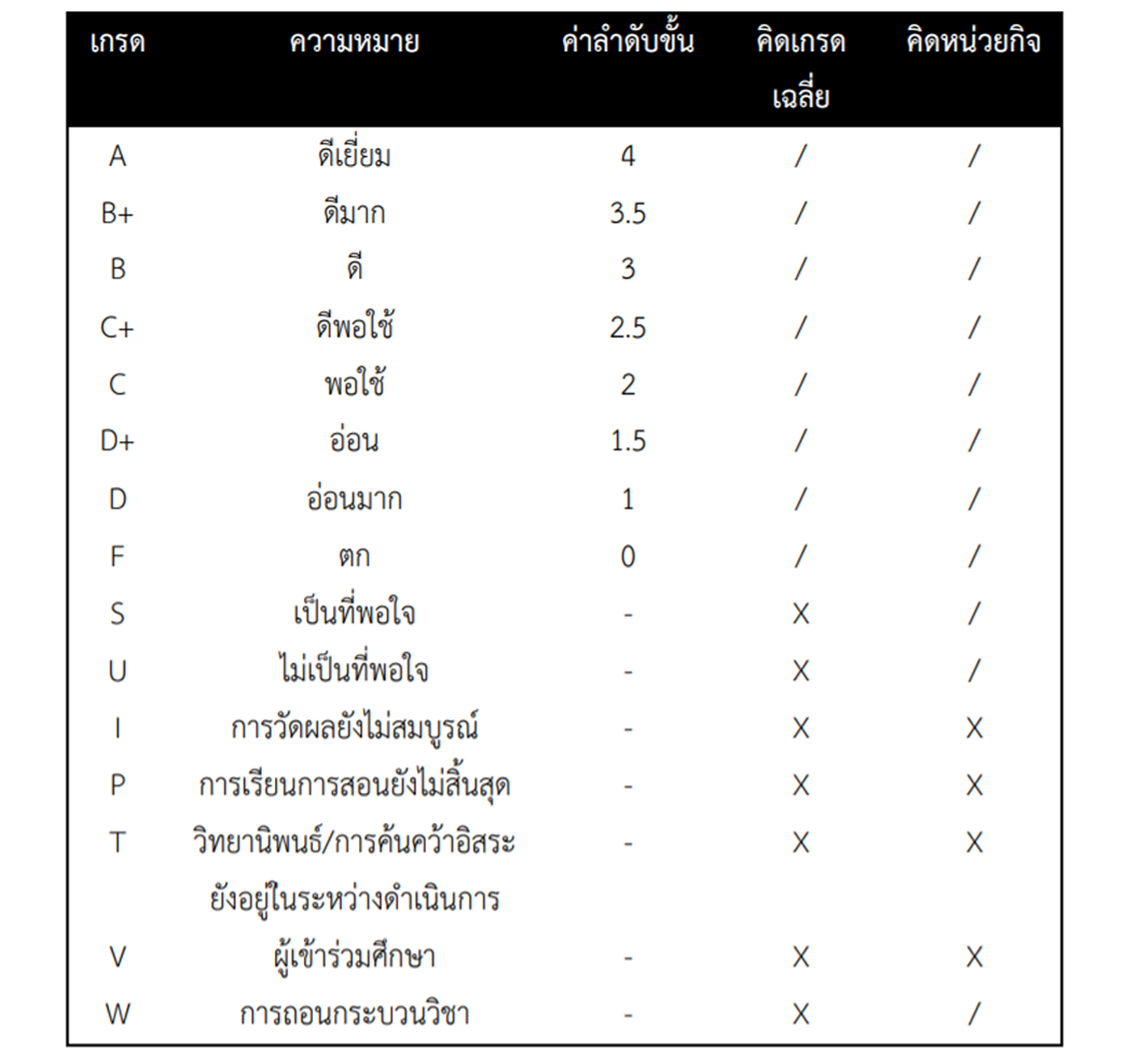
\includegraphics[width=1\textwidth]{table.png}
  \end{center}
  \caption {ตารางเเสดงเกรด}
  \end{figure}

\section{
เกณฑ์มาตรฐานหลักสูตรระดับปริญญาตรี พ.ศ. 2558 ตามประกาศของกระทรวงศึกษาธิการ
}

-โครงสร้างหลักสูตร

โดยตามประกาศของกระทรวงศึกษาธิการได้กล่าวถึงโครงสร้างของหลักสูตรในระดับปริญญาตรีไว้ดังนี้ว่า โครงสร้างหลักสูตร ต้องประกอบด้วยหมวดวิชาศึกษาทั่วไป หมวดวิชาเฉพาะ และหมวดวิชาเลือกเสรี โดยมีสัดส่วนจํานวนหน่วยกิตของแต่ละหมวดวิชา ดังนี้
\begin{enumerate}
    \item หมวดวิชาศึกษาทั่วไป หมายถึง หมวดวิชาที่เสริมสร้างความเป็นมนุษย์ที่สมบูรณ์ ให้มีความรอบรู้อย่างกว้างขวาง เข้าใจ และเห็นคุณค่าของตนเอง ผู้อื่น สังคม ศิลปวัฒนธรรม และธรรมชาติ ใส่ใจต่อความเปลี่ยนแปลงของสรรพสิ่ง พัฒนาตนเองอย่างต่อเนื่อง ดําเนินชีวิตอย่างมีคุณธรรม พร้อมให้ความช่วยเหลือเพื่อนมนุษย์ และเป็นพลเมืองที่มีคุณค่าของสังคมไทยและสังคมโลก 
    
    สถาบันอุดมศึกษาอาจจัดวิชาศึกษาทั่วไปในลักษณะจําแนกเป็นรายวิชาหรือลักษณะ บูรณาการใด ๆ ก็ได้ โดยผสมผสานเนื้อหาวิชาที่ครอบคลุมสาระของกลุ่มวิชาสังคมศาสตร์ มนุษยศาสตร์ ภาษาและกลุ่มวิชาวิทยาศาสตร์กับคณิตศาสตร์ ในสัดส่วนที่เหมาะสม เพื่อให้บรรลุวัตถุประสงค์ของ หมวดวิชาศึกษาทั่วไป โดยให้มีจํานวนหน่วยกิตรวมไม่น้อยกว่า 30 หน่วยกิต

    อนึ่ง การจัดวิชาศึกษาทั่วไปสําหรับหลักสูตรปริญญาตรี (ต่อเนื่อง) อาจได้รับการยกเว้น รายวิชาที่ได้ศึกษามาแล้วในระดับประกาศนียบัตรวิชาชีพชั้นสูงหรือระดับอนุปริญญา ทั้งนี้ จํานวนหน่วยกิต ของรายวิชาที่ได้รับการยกเว้นดังกล่าว เมื่อนับรวมกับรายวิชาที่จะศึกษาเพิ่มเติมในหลักสูตรปริญญาตรี (ต่อเนื่อง) ต้องไม่น้อยกว่า 30 หน่วยกิต
หมวดวิชาเฉพาะ หมายถึง วิชาแกน วิชาเฉพาะด้าน วิชาพื้นฐานวิชาชีพและวิชาชีพ ที่มุ่งหมายให้ผู้เรียนมีความรู้ ความเข้าใจ และปฏิบัติงานได้ โดยให้มีจํานวนหน่วยกิตรวม ดังนี้

    \item หมวดวิชาเฉพาะ หมายถึง วิชาแกน วิชาเฉพาะด้าน วิชาพื้นฐานวิชาชีพและวิชาชีพ ที่มุ่งหมายให้ผู้เรียนมีความรู้ ความเข้าใจ และปฏิบัติงานได้ โดยให้มีจํานวนหน่วยกิตรวม ดังนี้

    2.1 หลักสูตรปริญญาตรี (4 ปี) ทางวิชาการ ให้มีจํานวนหน่วยกิตหมวดวิชาเฉพาะ รวมไม่น้อยกว่า 72 หน่วยกิต
    2.2 หลักสูตรปริญญาตรี (4 ปี) ทางวิชาชีพหรือปฏิบัติการ ให้มีจํานวน หน่วยกิตหมวดวิชาเฉพาะรวมไม่น้อยกว่า 72 หน่วยกิต โดยต้องเรียนวิชาทางปฏิบัติการตามที่ มาตรฐานวิชาชีพกําหนด หากไม่มีมาตรฐานวิชาชีพกําหนดต้องเรียนวิชาทางปฏิบัติการไม่น้อยกว่า 36 หน่วยกิต และทางทฤษฎีไม่น้อยกว่า 24 หน่วยกิต

    หลักสูตร (ต่อเนื่อง) ให้มีจํานวนหน่วยกิตหมวดวิชาเฉพาะรวมไม่น้อยกว่า 42 หน่วยกิต ในจํานวนนั้นต้องเป็นวิชาทางทฤษฏีไม่น้อยกว่า 18 หน่วยกิต

    2.3	หลักสูตรปริญญาตรี (5 ปี) ให้มีจํานวนหน่วยกิตหมวดวิชาเฉพาะรวม ไม่น้อยกว่า 90 หน่วยกิต

    2.6 หลักสูตรปริญญาตรี (ไม่น้อยกว่า 6 ปี) ให้มีจํานวนหน่วยกิตหมวดวิชา เฉพาะรวมไม่น้อยกว่า 108 หน่วยกิต

    สถาบันอุดมศึกษาอาจจัดหมวดวิชาเฉพาะในลักษณะวิชาเอกเดี่ยว วิชาเอกคู่ หรือวิชาเอกและวิชาโทก็ได้ โดยวิชาเอกต้องมีจํานวนหน่วยกิตไม่น้อยกว่า 30 หน่วยกิต และวิชาโทต้องมีจํานวนหน่วยกิตไม่น้อยกว่า 15 หน่วยกิต ในกรณีที่จัดหลักสูตรแบบวิชาเอกคู่ต้องเพิ่ม จํานวนหน่วยกิตของวิชาเอกอีกไม่น้อยกว่า 30 หน่วยกิต และให้มีจํานวนหน่วยกิตรวมไม่น้อยกว่า 150 หน่วยกิต
		
    สําหรับหลักสูตรปริญญาตรีแบบก้าวหน้า ผู้เรียนต้องเรียนวิชาระดับ บัณฑิตศึกษาในหมวดวิชาเฉพาะไม่น้อยกว่า 12 หน่วยกิต 




    \item หมวดวิชาเลือกเสรี หมายถึง วิชาที่มุ่งให้ผู้เรียนมีความรู้ ความเข้าใจ ตามที่ ตนเองถนัดหรือสนใจ โดยเปิดโอกาสให้ผู้เรียนเลือกเรียนรายวิชาใด ๆ ในหลักสูตรระดับปริญญาตรี โดยให้มีจํานวนหน่วยกิตรวมไม่น้อยกว่า 6 หน่วยกิต
   
    สถาบันอุดมศึกษาอาจยกเว้นหรือเทียบโอนหน่วยกิตรายวิชาในหมวดวิชาศึกษาทั่วไป หมวดวิชาเฉพาะ และหมวดวิชาเลือกเสรี ให้กับนักศึกษาที่มีความรู้ความสามารถ ที่สามารถวัดมาตรฐานได้ ทั้งนี้ นักศึกษาต้องศึกษาให้ครบตามจํานวนหน่วยกิตที่กําหนดไว้ในเกณฑ์มาตรฐานหลักสูตร และเป็นไป ตามหลักเกณฑ์การเทียบโอนผลการเรียนระดับปริญญาเข้าสู่การศึกษาในระบบ และแนวปฏิบัติที่ดี เกี่ยวกับการเทียบโอน ของสํานักงานคณะกรรมการการอุดมศึกษา
  


-เกณฑ์การวัดผลและการสําเร็จการศึกษา

ให้สถาบันอุดมศึกษากําหนดเกณฑ์การวัดผล เกณฑ์ขั้นต่ําของแต่ละรายวิชา และเกณฑ์การสําเร็จการศึกษาตามหลักสูตร โดยต้องเรียนครบ ตามจํานวนหน่วยกิตที่กําหนดไว้ในหลักสูตร และต้องได้ระดับคะแนนเฉลี่ยไม่ตํ่ากว่า 2.00 จากระบบ 4 ระดับคะแนนหรือเทียบเท่า จึงถือว่าเรียนจบหลักสูตรปริญญาตรี 


\end{enumerate}

\section{ทฤษฎีความตัดกันของสี}

ในการออกแบบหน้าตาของ web application เพื่อให้เกิดความสวยงามนั้น จำเป็นที่จะต้องคำนึงถึงการเลือกใช้สีให้มีความเหมาะสมผู้ใช้งาน เพื่อไม่ให้สีนั้นเกิดความฉูดฉาดหรือเด่นชัดจนเกินไป รวมถึงไม่ให้สีดูกลมกลืนกันมากเกินไปด้วยเช่นกัน ดังนั้นผู้พัฒนาจึงใช้เว็บไซต์ชื่อ WebAIM : contrast Checker เพื่อเป็นตัวช่วยในการเทียบค่าความตัดกันของสีที่เลือกใช้ เช่น ไม่ให้สีของตัวหนังสือนั้นดูกลมกลืนกับพื้นหลังมากเกินไปจนผู้ใช้เกิดความยากลำบากในการอ่าน


\section{ทฤษฎีการเขียนโปรแกรมเชิงวัตถุ หรือ Object Oriented Programming (OOP)}

การเขียนโปรแกรมเชิงวัตถุ Object Oriented Programming (OOP) ก็คือการเขียนโปรแกรมเชิงวัตถุ ซึ่งเป็นแนวคิดในการพัฒนาซอฟแวร์ที่เป็นที่ยอมรับ เนื่องจากซอฟแวร์ที่ถูกพัฒนาและใช้กันอยู่นั้น นับวันมีแต่จะซับซ้อนมากยิ่งขึ้น ถ้าหากไม่จัดการกับโค้ดให้ดีพอก็อาจจะทำให้การพัฒนาล่าช้าหรือไม่สำเร็จได้  OOP จึงออกแบบมาให้โค้ดที่เราเขียนมีแบบแผนที่เหมาะสมพร้อมใช้ในการพัฒนาที่ซับซ้อนได้ โดยมองสิ่งต่างๆในระบบเป็นวัตถุ (Object) ชิ้นหนึ่งที่มีหน้าที่และความหมายในตัว โดยวัตถุๆนั้น ก็มี คุณสมบัติ (Attributes) และ พฤติกรรม (Method,Behavior) หรือการกระทำของมัน เป็นการมองบนพื้นฐานความเป็นจริงมากขึ้น นอกจากนี้ยังมี 4 หลักสําคัญของ OOP อยู่ด้วยได้แก่

\begin{enumerate}

\item Encapsulation : ห่อหุ้มค่าของสิ่งต่างๆไว้ แก้ไขหรือเข้าถึงได้ผ่าน Method
\item Inheritance : สืบทอด Attributes และ Method จากคลาสแม่โดยสามารถเพิ่มได้
\item Polymorphism : Object จาก Class เดียวกันมีผลลัพธ์ของ Method ต่างกัน
\item Abstaction : เป็นแบบร่างคร่าวๆให้พอรู้ โดยยังไม่สนใจวิธีการทำงาน


\end{enumerate}
\chapter{\ifproject%
\ifenglish Project Structure and Methodology\else โครงสร้างและขั้นตอนการทำงาน\fi
\else%
\ifenglish Project Structure\else โครงสร้างของโครงงาน\fi
\fi
}

ในบทนี้จะกล่าวถึงหลักการ และการออกแบบระบบ

\makeatletter

% \renewcommand\section{\@startsection {section}{1}{\z@}%
%                                    {13.5ex \@plus -1ex \@minus -.2ex}%
%                                    {2.3ex \@plus.2ex}%
%                                    {\normalfont\large\bfseries}}

\makeatother
%\vspace{2ex}
% \titleformat{\section}{\normalfont\bfseries}{\thesection}{1em}{}
% \titlespacing*{\section}{0pt}{10ex}{0pt}

\section{Alice in Wonderland}

\begin{figure}
\begin{center}
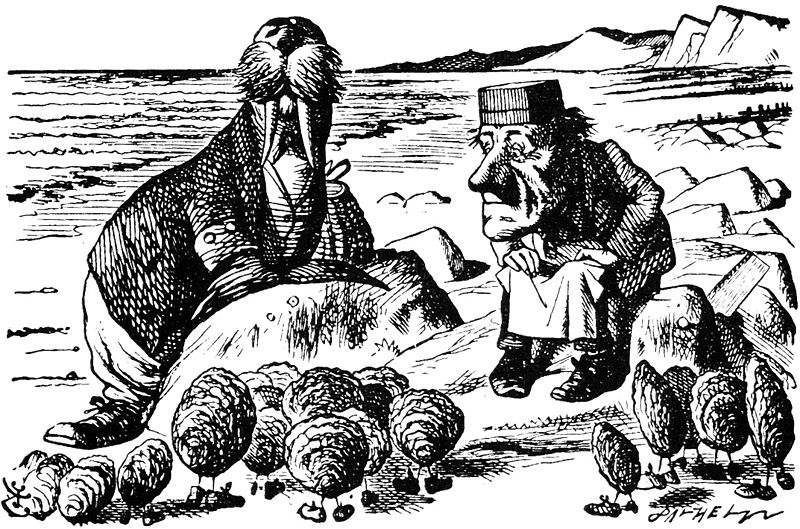
\includegraphics{800px-Briny_Beach.jpg}
\end{center}
\caption[Poem]{The Walrus and the Carpenter}
\label{fig:walrus}
\end{figure}

\subsection{The Black Kitten}
  One thing was certain, that the WHITE kitten had had nothing to
do with it:---it was the black kitten's fault entirely~\cite{aiw}.  For the
white kitten had been having its face washed by the old cat for
the last quarter of an hour (and bearing it pretty well,
considering); so you see that it COULDN'T have had any hand in
the mischief.

  The way Dinah washed her children's faces was this:  first she
held the poor thing down by its ear with one paw, and then with
the other paw she rubbed its face all over, the wrong way,
beginning at the nose:  and just now, as I said, she was hard at
work on the white kitten, which was lying quite still and trying
to purr---no doubt feeling that it was all meant for its good.

  But the black kitten had been finished with earlier in the
afternoon, and so, while Alice was sitting curled up in a corner
of the great arm-chair, half talking to herself and half asleep,
the kitten had been having a grand game of romps with the ball of
worsted Alice had been trying to wind up, and had been rolling it
up and down till it had all come undone again; and there it was,
spread over the hearth-rug, all knots and tangles, with the
kitten running after its own tail in the middle.

\subsection{The Reproach}

  `Oh, you wicked little thing!' cried Alice, catching up the
kitten, and giving it a little kiss to make it understand that it
was in disgrace.  `Really, Dinah ought to have taught you better
manners!  You OUGHT, Dinah, you know you ought!' she added,
looking reproachfully at the old cat, and speaking in as cross a
voice as she could manage---and then she scrambled back into the
arm-chair, taking the kitten and the worsted with her, and began
winding up the ball again.  But she didn't get on very fast, as
she was talking all the time, sometimes to the kitten, and
sometimes to herself.  Kitty sat very demurely on her knee,
pretending to watch the progress of the winding, and now and then
putting out one paw and gently touching the ball, as if it would
be glad to help, if it might.

  `Do you know what to-morrow is, Kitty?' Alice began.  `You'd
have guessed if you'd been up in the window with me---only Dinah
was making you tidy, so you couldn't.  I was watching the boys
getting in stick for the bonfire---and it wants plenty of
sticks, Kitty!  Only it got so cold, and it snowed so, they had
to leave off.  Never mind, Kitty, we'll go and see the bonfire
to-morrow.'  Here Alice wound two or three turns of the worsted
round the kitten's neck, just to see how it would look:  this led
to a scramble, in which the ball rolled down upon the floor, and
yards and yards of it got unwound again.

  `Do you know, I was so angry, Kitty,' Alice went on as soon as
they were comfortably settled again, `when I saw all the mischief
you had been doing, I was very nearly opening the window, and
putting you out into the snow!  And you'd have deserved it, you
little mischievous darling!  What have you got to say for
yourself?  Now don't interrupt me!' she went on, holding up one
finger.  `I'm going to tell you all your faults.  Number one:
you squeaked twice while Dinah was washing your face this
morning.  Now you can't deny it, Kitty:  I heard you!  What that
you say?' (pretending that the kitten was speaking.)  `Her paw
went into your eye?  Well, that's YOUR fault, for keeping your
eyes open---if you'd shut them tight up, it wouldn't have
happened.  Now don't make any more excuses, but listen!  Number
two:  you pulled Snowdrop away by the tail just as I had put down
the saucer of milk before her!  What, you were thirsty, were you?

\chapter{\ifproject%
\ifenglish Experimentation and Results\else การทดลองและผลลัพธ์\fi
\else%
\ifenglish System Evaluation\else การประเมินระบบ\fi
\fi}

ในบทนี้จะทดสอบเกี่ยวกับการทำงานในฟังก์ชันหลักๆ

\ifproject
\chapter{\ifenglish Conclusions and Discussions\else บทสรุปและข้อเสนอแนะ\fi}

\section{\ifenglish Conclusions\else สรุปผล\fi}

นศ. ควรสรุปถึงข้อจำกัดของระบบในด้านต่างๆ ที่ระบบมีในเนื้อหาส่วนนี้ด้วย

\section{\ifenglish Challenges\else ปัญหาที่พบและแนวทางการแก้ไข\fi}

ในการทำโครงงานนี้ พบว่าเกิดปัญหาหลักๆ ดังนี้

\section{\ifenglish%
Suggestions and further improvements
\else%
ข้อเสนอแนะและแนวทางการพัฒนาต่อ
\fi
}

ข้อเสนอแนะเพื่อพัฒนาโครงงานนี้ต่อไป มีดังนี้

\fi

\bibliography{sampleReport}

\ifproject
\appendix
\chapter{The first appendix}

Text for the first appendix goes here.

\section{Appendix section}

Text for a section in the first appendix goes here.

test ทดสอบฟอนต์ serif ภาษาไทย

\textsf{test ทดสอบฟอนต์ sans serif ภาษาไทย}

\verb+test ทดสอบฟอนต์ teletype ภาษาไทย+

\texttt{test ทดสอบฟอนต์ teletype ภาษาไทย}

\textbf{ตัวหนา serif ภาษาไทย \textsf{sans serif ภาษาไทย} \texttt{teletype ภาษาไทย}}

\textit{ตัวเอียง serif ภาษาไทย \textsf{sans serif ภาษาไทย} \texttt{teletype ภาษาไทย}}

\textbf{\textit{ตัวหนาเอียง serif ภาษาไทย \textsf{sans serif ภาษาไทย} \texttt{teletype ภาษาไทย}}}

\url{https://www.example.com/test_ทดสอบ_url}

\chapter{\ifenglish Manual\else คู่มือการใช้งานระบบ\fi}

Manual goes here.


%% Display glossary (optional) -- need glossary option.
\ifglossary\glossarypage\fi

%% Display index (optional) -- need idx option.
\ifindex\indexpage\fi

\begin{biosketch}
\begin{center}
  
\includegraphics[width=1.5in]{mugshot.jpg}
\end{center}
Your biosketch goes here. Make sure it sits inside
the \texttt{biosketch} environment.
\end{biosketch}
\fi % \ifproject
\end{document}
